% Problem 1 - Superposition (10 points)
\Point{superposition}{calculatevab}{10}
\Point{superposition}{compare}{2}
\begin{mainquestion}{superposition}{Superposition}
Consider this circuit that you've solved in a previous assignment:

\begin{center}
    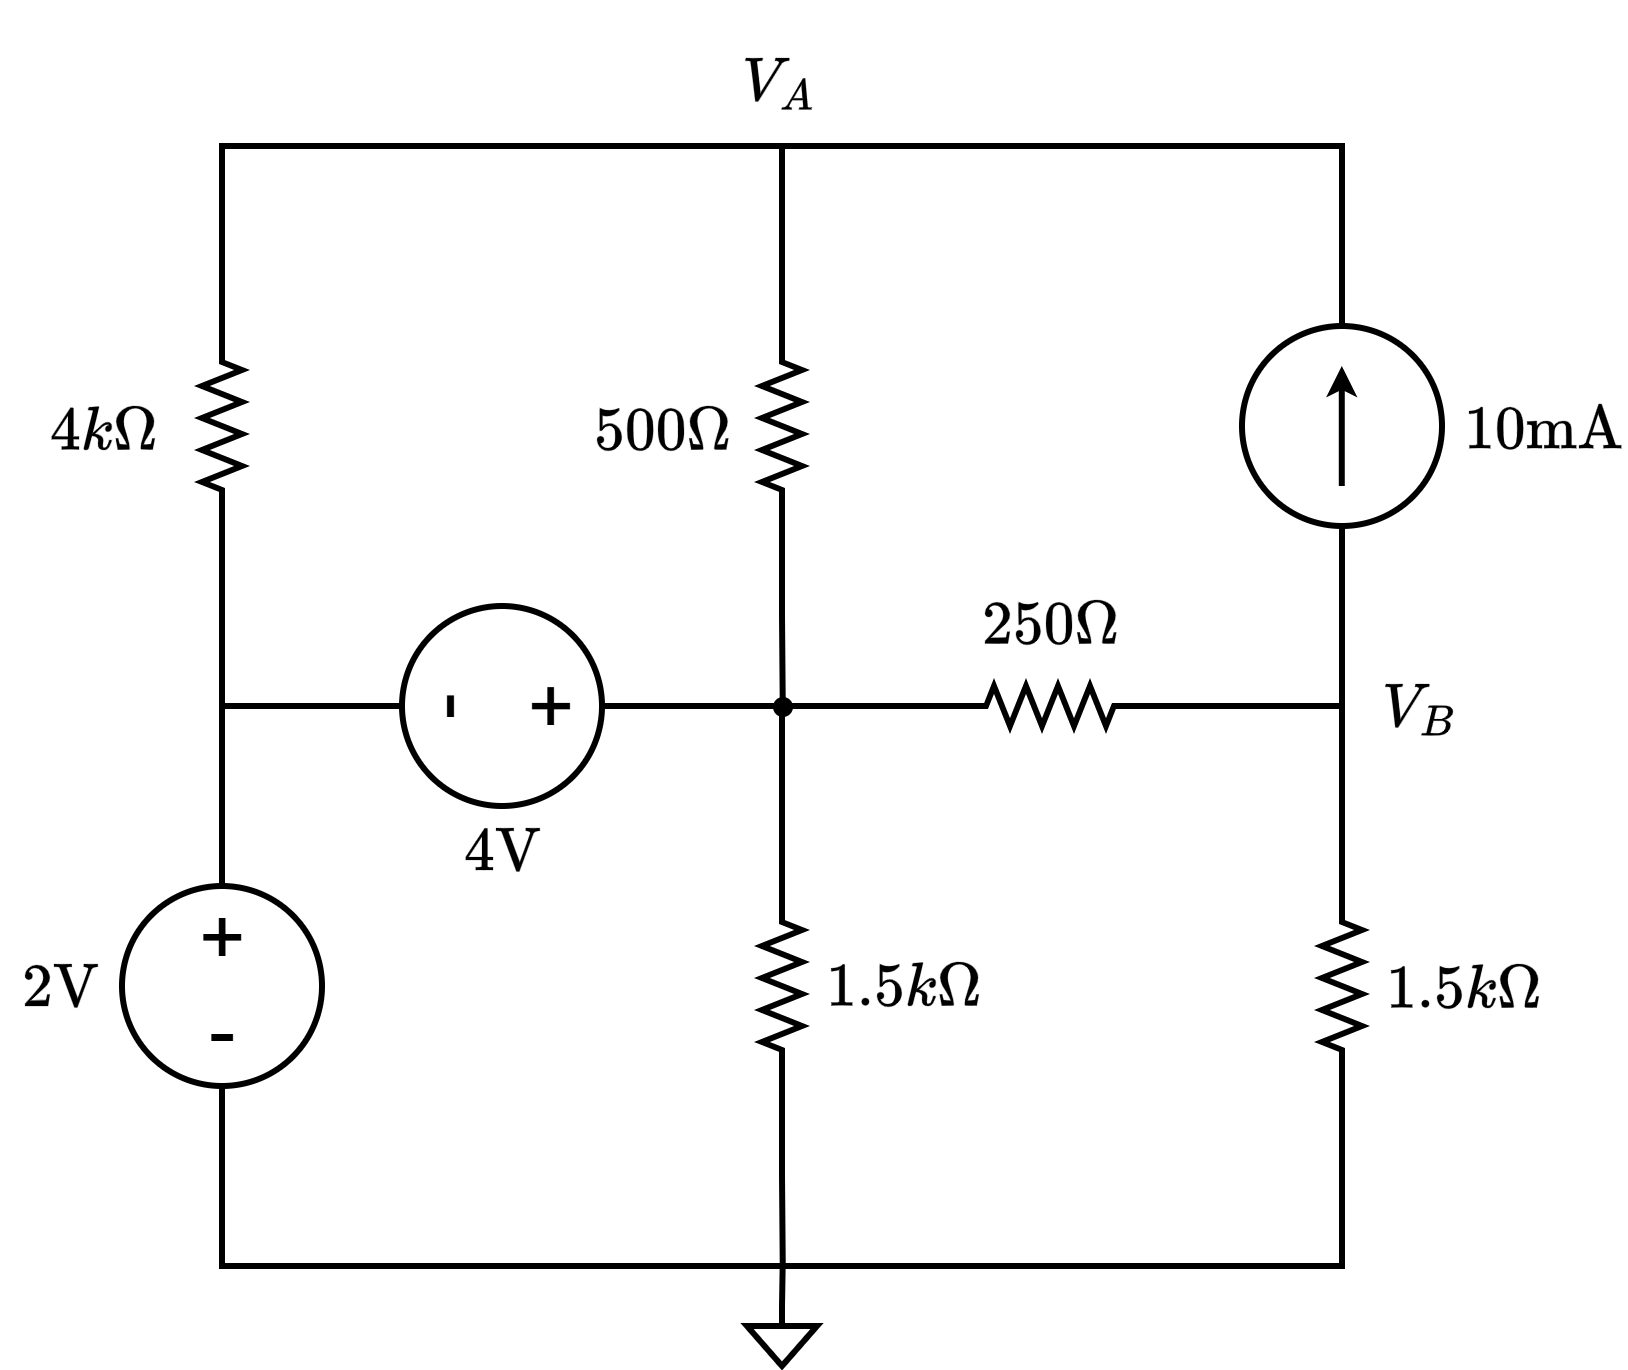
\includegraphics[width=0.8\textwidth]{questionbank/networks/superposition/v1/schematic.png}
\end{center}

\begin{partquestion}{calculatevab}{Use superposition to find $V_A$ and $V_B$.}
\begin{answer}
Superposition tells us that we can consider the effect of each independent source individually. We can do this by disabling all but one of the independent sources (open current sources, short voltage sources) and solving for the voltages at $V_A$ and $V_B$. Then we can add up the contributions to each and we should get the final values of $V_A$ and $V_B$, respectively.
\bigskip

\textbf{2V source only:} open the 10 mA source and short the 4 V source. The circuit becomes:
\begin{center}
    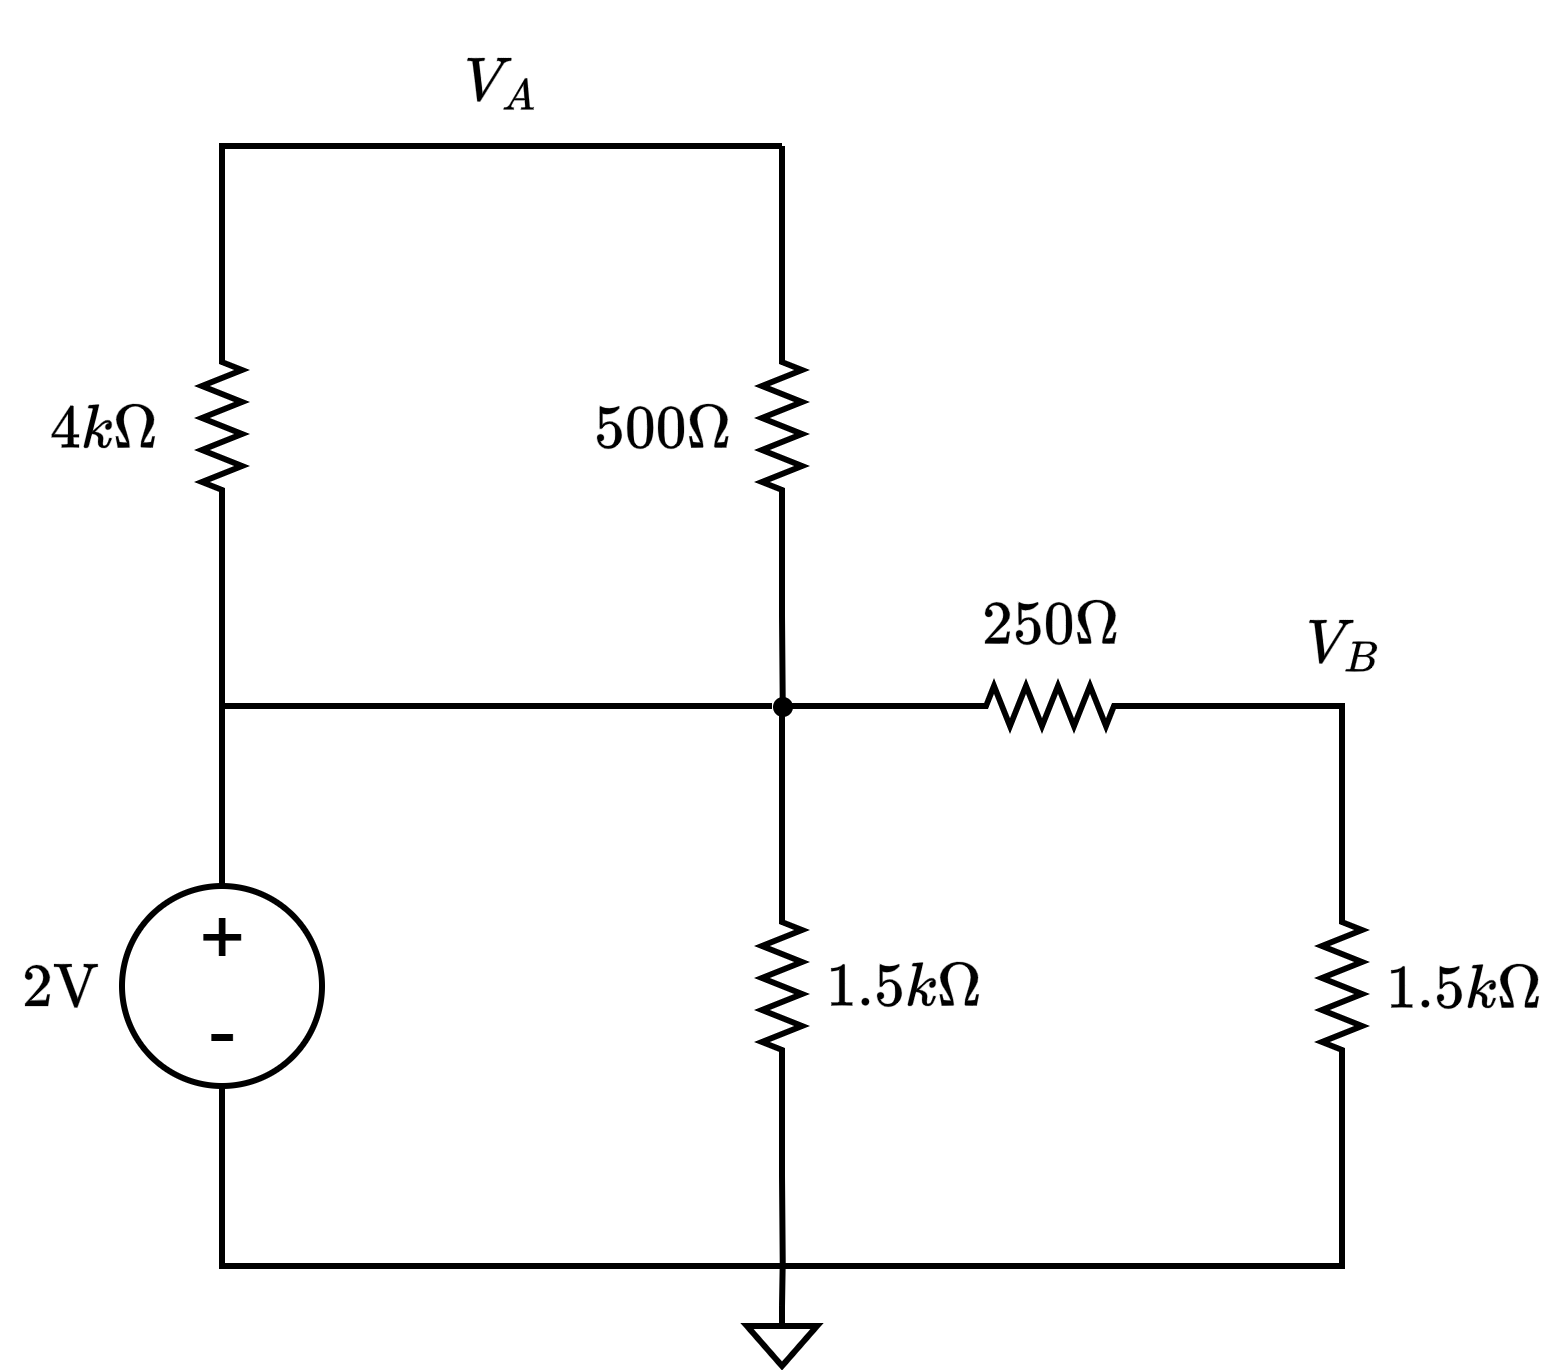
\includegraphics[width=0.6\textwidth]{questionbank/networks/superposition/v1/super_2v.png}
\end{center}

The circuit is now just a resistor network with a single independent source. We see right away that $V_B$ is the output of a voltage divider:
\[
V_B = 2\frac{1500}{1500 +250} = \frac{12}{7}\unit{\volt}
\]
$V_A$ is stranded at the top of the circuit. KVL tells us that the drop across the \qty{4}{\kilo\ohm} resistor and the \qty{500}{\ohm} must add up to zero, but parallel elements must have the same voltage:
\[
V_{4k\Omega} + V_{500\Omega} = 0 \hspace{1cm} V_{4k\Omega} = V_{500\Omega}
\]

The only solution is if $V_{4k\Omega}$ and $V_{500\Omega}$ are both \qty{0}{\volt}! This implies that $V_A$ is the same voltage as the voltage source, so:
\[V_A = \qty{2}{\volt}\]
\bigskip

\textbf{4 V source only:} open the 10 mA source and short the 2 V source. The circuit becomes:
\begin{center}
    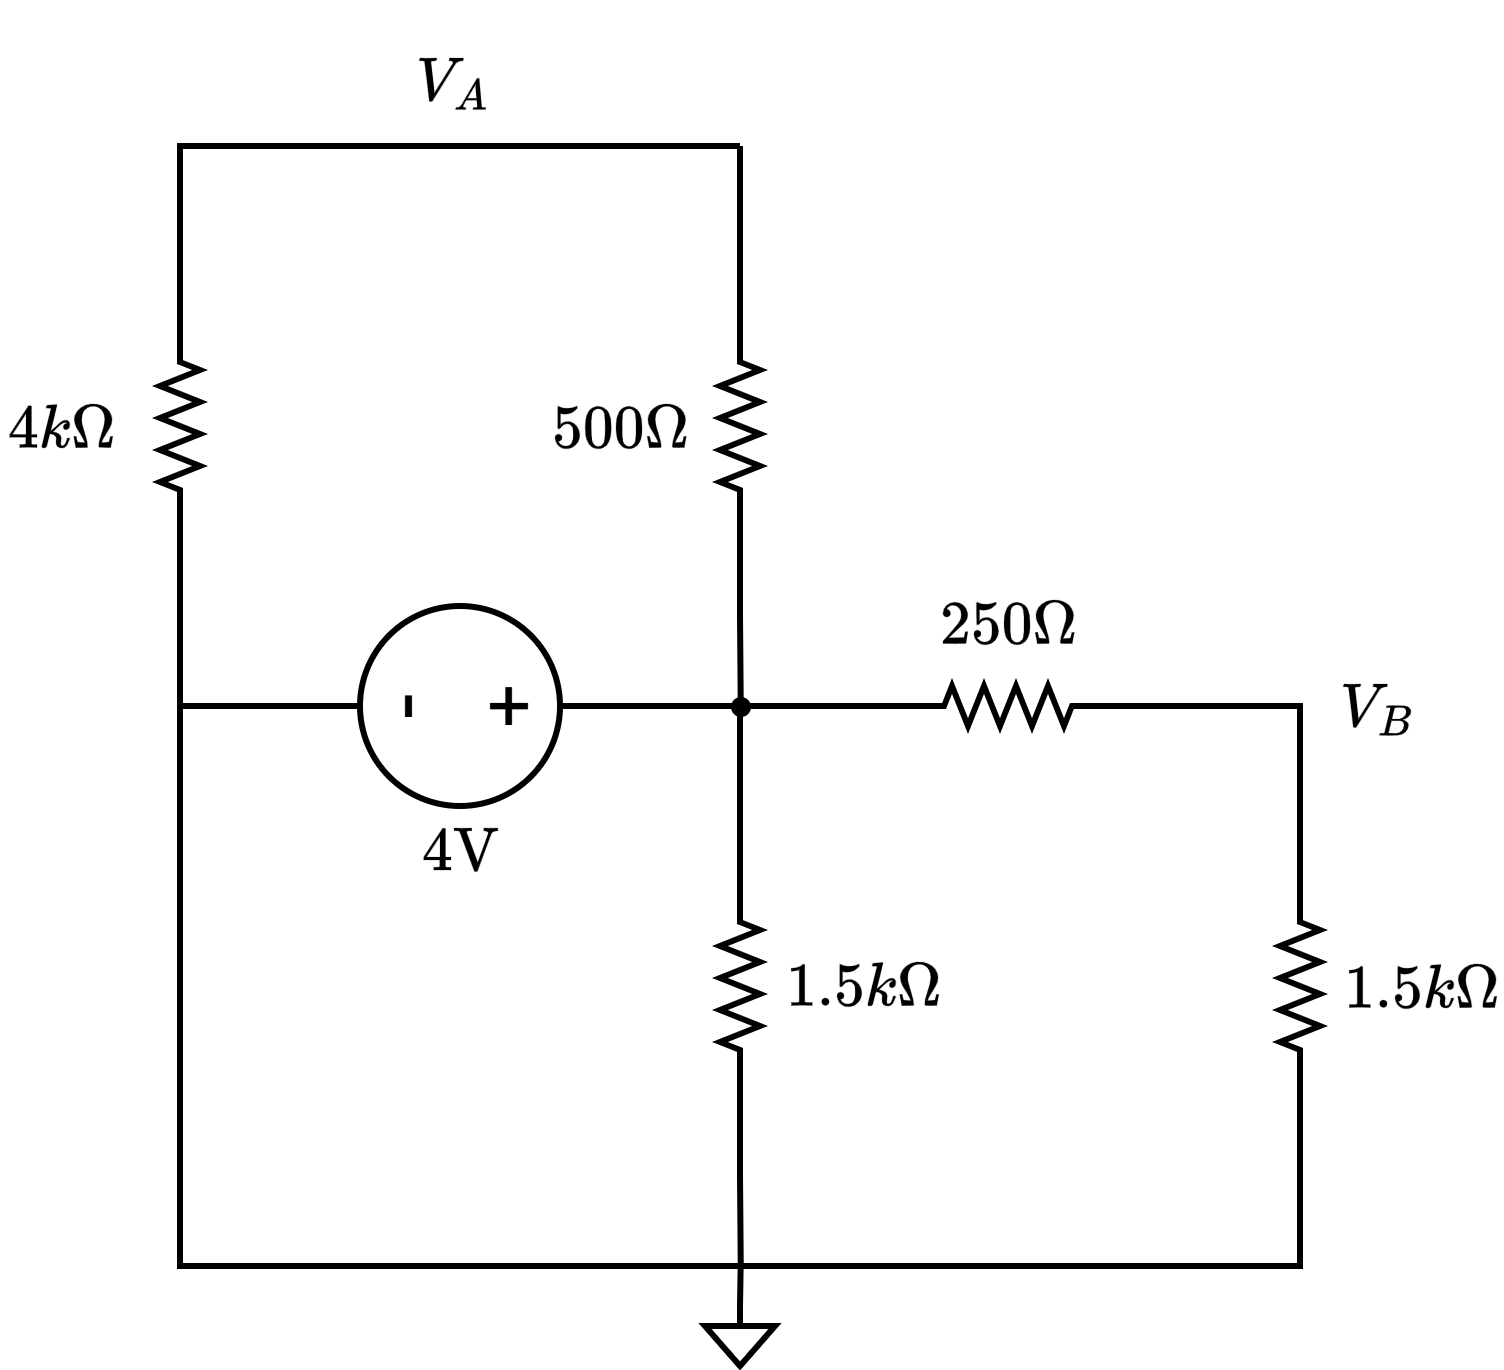
\includegraphics[width=3in]{questionbank/networks/superposition/v1/super_4v.png}
\end{center}

This is very similar to before, except now both $V_A$ and $V_B$ are voltage dividers:
\[
V_A = 4\frac{4000}{4000 +500} = \frac{32}{9}\unit{\volt}
\]

\[
V_B = 4\frac{1500}{1500 +250} = \frac{24}{7}\unit{\volt}
\]
\bigskip

\textbf{10 mA source only:} short both voltage sources. The circuit becomes:
\begin{center}
    \includegraphics[width=3in]{questionbank/networks/superposition/v1/super_10mA.png}
\end{center}

Let's take a second to figure out what we are looking at. The current from our 10mA source will pass through the \qty{4}{\kilo\ohm} resistor and the \qty{500}{\ohm} resistor in parallel before reaching ground. Then the current will pass through the \qty{1.5}{\kilo\ohm} resistor and the \qty{250}{\ohm} resistor in parallel on its way back to the current source. The other \qty{1.5}{\kilo\ohm} is shorted so the current won't bother to flow through it.

The voltages $V_A$ and $V_B$ will be the voltage drops across the effective parallel resistor pairs:

\[V_A = 10 \frac{0.5 \cdot 4}{4 + 0.5} = \frac{40}{9}\unit{\volt}\]
\[V_B = -10 \frac{0.25 \cdot 1.5}{1.5 + 0.25} = -\frac{15}{7}\unit{\volt}\]
Note $V_B$ is negative thanks to our passive sign convention.
\bigskip

Now we can sum our results to find the final values:
\[
V_A = 2 + \frac{32}{9} + \frac{40}{9} = \frac{90}{9} = \qty{10}{\volt}
\]
\[
V_B = \frac{12}{7} + \frac{24}{7} - \frac{15}{7} = \frac{21}{7} = \qty{3}{\volt}
\]
\end{answer}
\end{partquestion}

\begin{partquestion}{compare}{Does your result in part (\cref{prob:superposition:calculatevab}) match your solution from HW2 Problem 1? Which method do you prefer and why?}

\begin{answer}
    Our solution to HW2 Problem 1 found that the voltage across $R_5$ (rightmost \qty{1.5}{\kilo\ohm}) was \qty{3}{\volt} and the voltage across $R_1$ (upper right \qty{4}{\kilo\ohm}) was \qty{8}{\volt}. Given we assign the bottom node to be ground as shown, that would imply $V_A = 2 + 8 = \qty{10}{\volt}$ and $V_B = \qty{3}{\volt}$, a perfect match!
    In this case superposition made our job easier by removing the need to solve any systems of equations.
\end{answer}
\end{partquestion}

\end{mainquestion}


% Problem 2 - Thevenin Equivalent (20 points)
\clearpage
\Point{thevenin_meas}{missingdata}{2}
\Point{thevenin_meas}{suspiciousdata}{3}
\Point{thevenin_meas}{iandv}{7}
\Point{thevenin_meas}{equation}{2}
\Point{thevenin_meas}{rload}{2}
\Point{thevenin_meas}{maxpower}{4}
\begin{mainquestion}{thevenin_meas}{Measuring Thévenin}
A black box filled with linear circuitry is connected to a variable resistor.  An ideal ammeter (with zero resistance) and an ideal voltmeter (with infinite resistance) are used to measure current and voltage as shown below. The results of several sample readings are listed in the accompanying table.

\begin{table}[htbp]
\centering
\label{tab:measurements}
\begin{tabular}{|c | c |  c|}
\hline
\textbf{R ($\Omega$)} & \textbf{V (volts)} & \textbf{I (amps)} \\
\hline
4 &  & 1.5 \\ \hline
6 & 8 & \\ \hline
 & 9.6 & 1.2 \\ \hline
10 &  & 1 \\ \hline

\end{tabular}
\end{table}

\begin{partquestion}{missingdata}{Based on what you see in the table, fill in the missing values.}
\begin{answer}
Using Ohm's Law, $V=IR$ and we can determine the missing values:
\begin{table}[htbp]
\centering
\label{tab:measurementsfilled}
\begin{tabular}{|c | c |  c|}
\hline
\textbf{R ($\Omega$)} & \textbf{V (volts)} & \textbf{I (amps)} \\
\hline
4 & 6 & 1.5 \\ \hline
6 & 8 & 1.333\\ \hline
8 & 9.6 & 1.2 \\ \hline
10 & 10  & 1 \\ \hline
\end{tabular}
\end{table}
\end{answer}
\end{partquestion}

\begin{partquestion}{suspiciousdata}{It appears there is some suspicious data in the above table. Plot an estimate of the load line.  Can you determine which data row is wrong?  How do you know?}
\begin{answer}
For any linear system, plotting these data points on an I-V curve should result in a straight line.
\begin{center}
    \includegraphics[width=4in]{figure.png}
\end{center}
We can see that there is one data point which is not co-linear with the other three; this point at (10 V, 1 A) must be invalid data.
\end{answer}
\end{partquestion}
\begin{partquestion}{iandv}{Find $I$ and $V$ when $R=\qty{17}{\ohm}$.}
\begin{answer}
Replace the black box by its Th\'evenin equivalent, consisting of a source $V_{\mathrm{th}}$ in series with a resistance $R_{\mathrm{th}}$. For a load
  resistance $R$,
  \[
    \frac{V}{V_{\mathrm{th}}}=\frac{R}{R+R_{\mathrm{th}}}.
  \]
  Using the measurements for $R=\qty{4}{\ohm}$ and $R=\qty{6}{\ohm}$ gives
  \[
    \frac{6}{V_{\mathrm{th}}}=\frac{4}{4+R_{\mathrm{th}}},
    \qquad
    \frac{8}{V_{\mathrm{th}}}=\frac{6}{6+R_{\mathrm{th}}}.
  \]
  Eliminating $V_{\mathrm{th}}$,
  \begin{align*}
    \frac{6}{4}(4+R_{\mathrm{th}})
      &= \frac{8}{6}(6+R_{\mathrm{th}}),\\
    6+\frac{3}{2}R_{\mathrm{th}}
      &= 8+\frac{4}{3}R_{\mathrm{th}},\\
    R_{\mathrm{th}} &= \qty{12}{\ohm}.
  \end{align*}
  It follows that
  \[
    V_{\mathrm{th}}
      =\frac{6}{4}(4+12)
      =\qty{24}{\volt}.
  \]
  Therefore, with $R=\qty{17}{\ohm}$,
  \[
    V=V_{\mathrm{th}}\frac{R}{R+R_{\mathrm{th}}}
      =24\frac{17}{17+12}
      =\frac{408}{29}\,\mathrm{V}
      \approx \qty{14.1}{\volt},
  \]
  and
  \[
    I=\frac{V}{R}
      =\frac{24}{29}\,\mathrm{A}
      \approx \qty{0.83}{\ampere}.
  \]
\end{answer}
\end{partquestion}
\begin{partquestion}{equation}{With your results from (\cref{prob:thevenin_meas:iandv}), now determine the exact equation for the load line sketched in (\cref{prob:thevenin_meas:suspiciousdata}) }
\begin{answer}
The equation is:
\[
    I=-\frac{V}{R_\mathrm{th}}+\frac{V_\mathrm{th}}{R_\mathrm{th}}
      =-\frac{V}{12}+2
  \]
\end{answer}
\end{partquestion}
\begin{partquestion}{rload}{Determine the value of $R$ that achieves maximum power transfer from the black box to the variable resistor.}
\begin{answer}
Maximum power transfer occurs when the load resistance equals the Th\'evenin
  resistance:
  \[
    \boxed{R=R_{\mathrm{th}}=\qty{12}{\ohm}.}
  \]
\end{answer}
\end{partquestion}
\begin{partquestion}{maxpower}{What is the maximum power transferred to the variable resistor?}
\begin{answer}
 With $R=R_{\mathrm{th}}$, the maximum load power is
  \[
    P_{\max}=\frac{V_{\mathrm{th}}^2}{4R_{\mathrm{th}}}
      =\frac{(\qty{24}{\volt})^2}{4(\qty{12}{\ohm})}
      =\boxed{\qty{12}{\watt}}.
  \]
\end{answer}
\end{partquestion}

\end{mainquestion}

% Problem 3 - Ammeter Connection and Equivalent Circuits (16 points)
\clearpage
\Point{ammeter}{connection}{3}
\Point{ammeter}{thevenin}{5}
\Point{ammeter}{norton}{3}
\Point{ammeter}{ri300}{2}
\Point{ammeter}{ri0}{2}
\Point{ammeter}{rimax}{3}
\begin{mainquestion}{ammeter}{Equivalent Circuits}
Consider the circuit shown below. An ammeter with an internal resistance of $R_{i}$ is used to measure the current flowing through a 560$\Omega$ resistor between points $A$ and $B$.

\begin{center}
    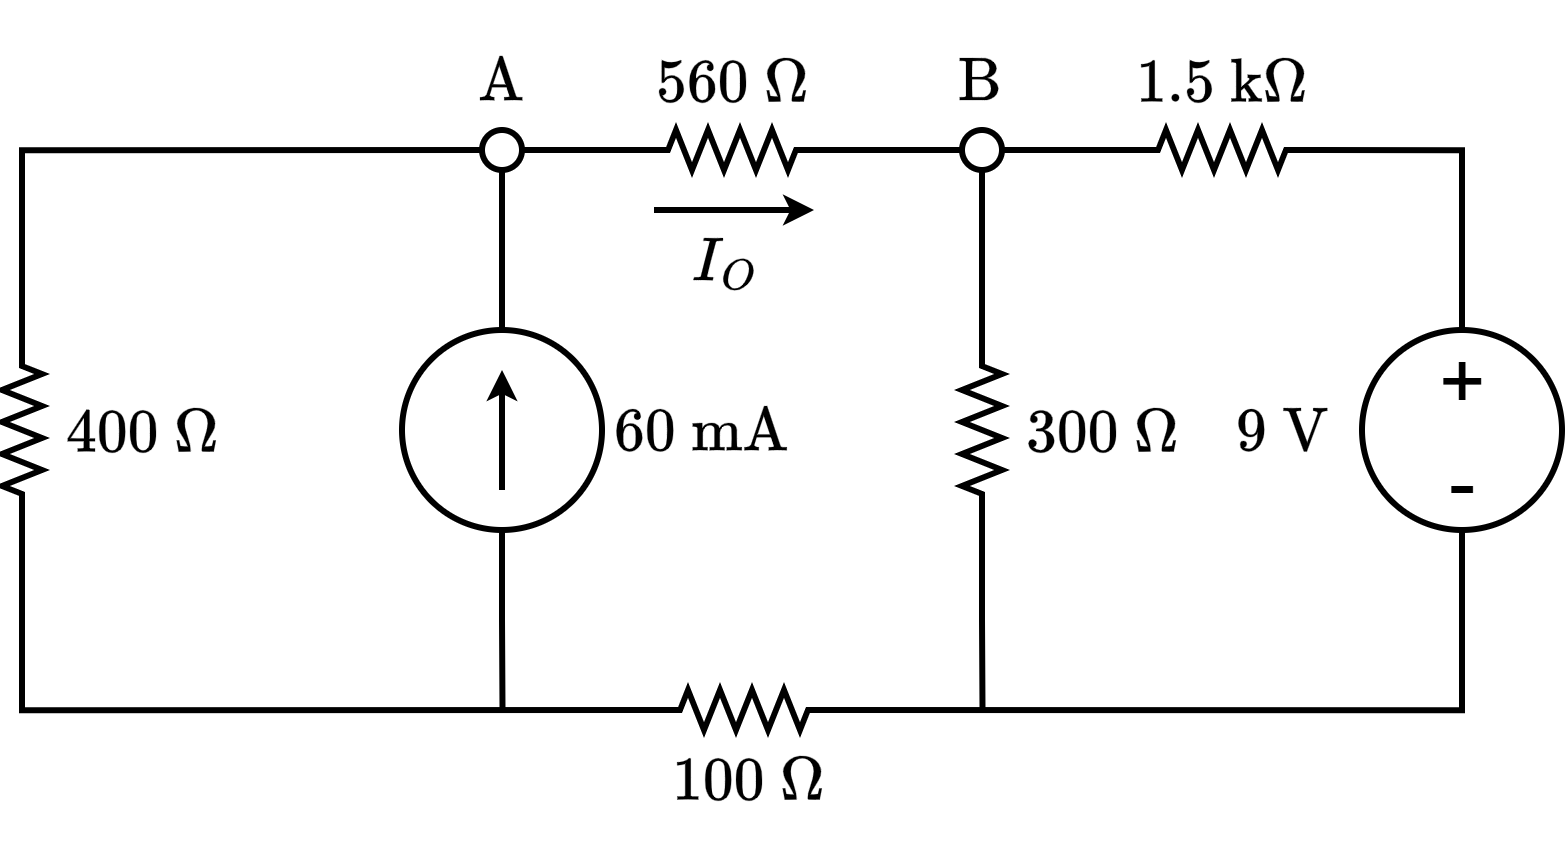
\includegraphics[width=5in]{questionbank/networks/ammeter_thevenin_norton/v1/circuit.png}
\end{center}

\begin{partquestion}{connection}{How should the ammeter be connected between $A$ and $B$? Show a sketch of the circuit (only include the portion between $A$ and $B$) which includes the ammeter with its internal resistance.}
\begin{answer}
The ammeter should be connected in series with the 560$\Omega$ resistor between terminals $A$ and $B$. This means the current through the load passes through the ammeter and its internal resistance.

\begin{center}
    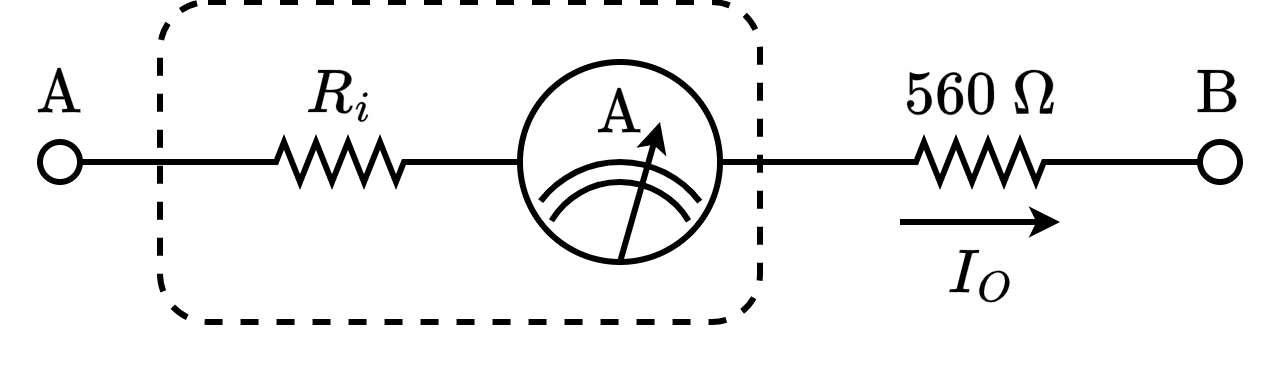
\includegraphics[width=0.7\textwidth]{questionbank/networks/ammeter_thevenin_norton/v1/ammeter_conn.png}
\end{center}
\end{answer}
\end{partquestion}

\begin{partquestion}{thevenin}{Find the Thévenin equivalent circuit at terminals $A$ and $B$ (without the 560$\Omega$ load).}
\begin{answer}
To find the Thévenin resistance, we zero out all independent sources. The current source becomes an open circuit and the voltage source becomes a short circuit:

\begin{center}
    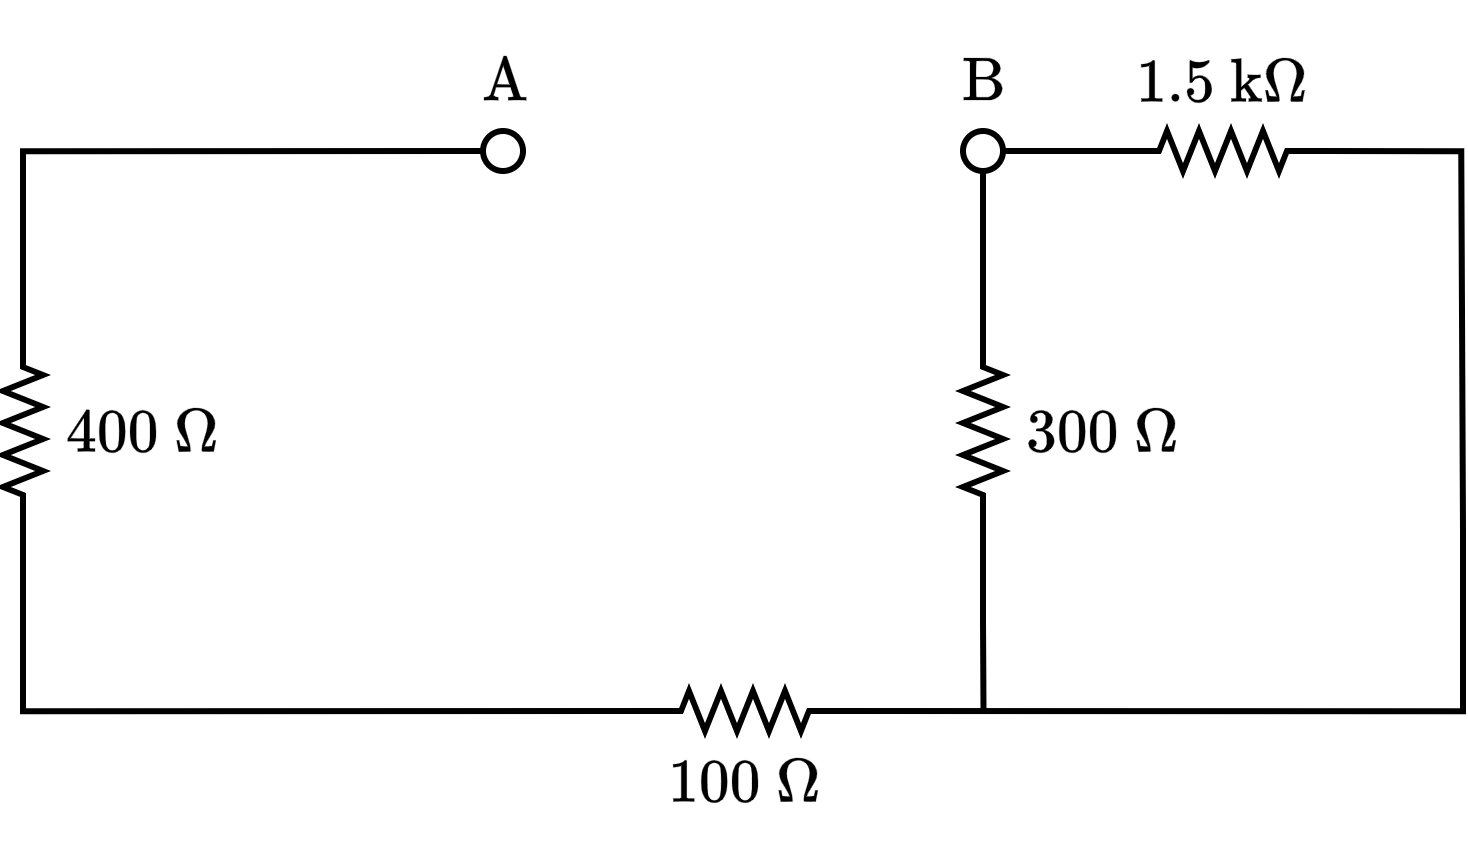
\includegraphics[width=0.7\textwidth]{questionbank/networks/ammeter_thevenin_norton/v1/rthev.png}
\end{center}

We can now combine the remaining resistors to find a single equivalent resistance.

\begin{align*}
    R_{TH} &= \qty{400}{\ohm} + \qty{100}{\ohm} + \qty{300}{\ohm}||\qty{1.5}{\kilo\ohm} \\
    &= \qty{500}{\ohm} + \frac{0.3\cdot1.5}{0.3+1.5}\unit{\kilo\ohm} \\
    &= \qty{750}{\ohm} \\
\end{align*}

\begin{center}
    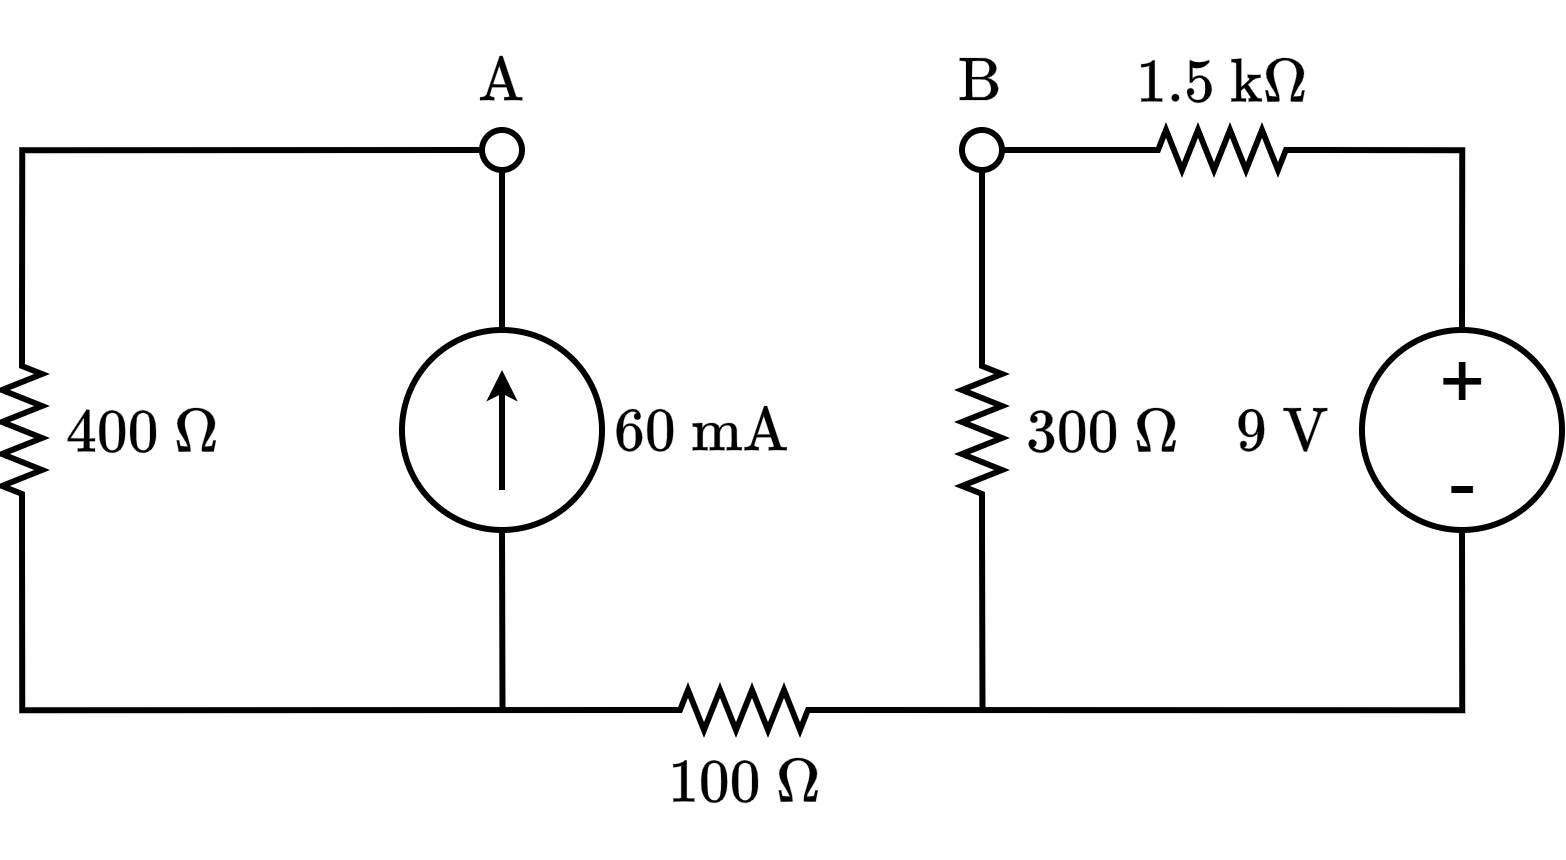
\includegraphics[width=4.5in]{questionbank/networks/ammeter_thevenin_norton/v1/thev_start.png}
\end{center}

Now to find the Thévenin voltage, compute the open-circuit voltage at $A$ and $B$. Because no current flows through the 100$\Omega$ branch, its voltage is zero. The open-circuit voltage measured from $A$ to $B$ is therefore the voltage drop across the current source ($\qty{60}{\milli\ampere} \cdot\qty{400}{\ohm} = \qty{24}{\volt}$) minus the output of the voltage divider formed from the \qty{1.5}{\kilo\ohm} and \qty{300}{\ohm} resistors with the 9 V source ($9 \frac{3}{3+15} = \qty{1.5}{\volt}$). Thus $V_{\text{TH}} = 24 - 1.5 = 22.5~\text{V}$.

Now that we have both the Thévenin voltage and Thévenin resistance, we can combine them to find our equivalent circuit:

\begin{center}
    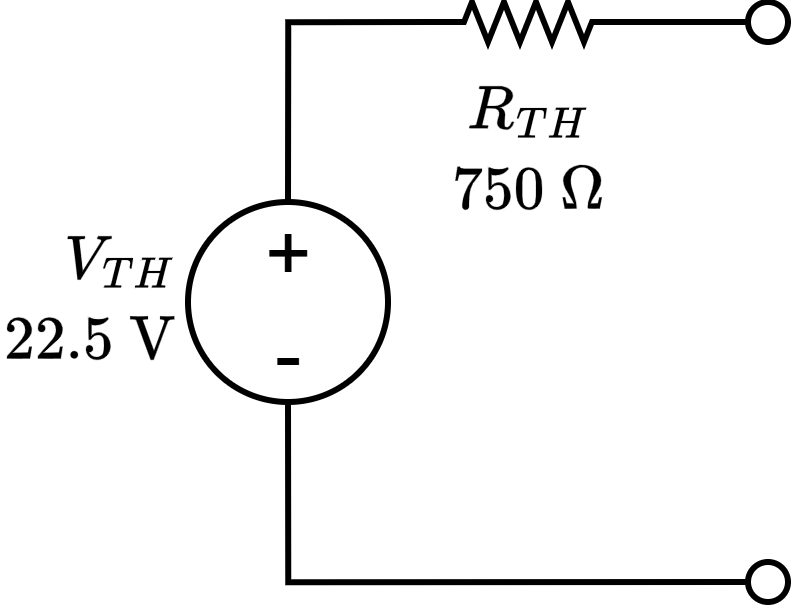
\includegraphics[width=2in]{questionbank/networks/ammeter_thevenin_norton/v1/thev_eq.png}
\end{center}
\end{answer}
\end{partquestion}

\begin{partquestion}{norton}{Find the Norton equivalent circuit at terminals $A$ and $B$ (without the 560$\Omega$ load).}
\begin{answer}
Using the previously computed Thévenin equivalent, the Norton current is $I_{N} = V_{\text{TH}} / R_{\text{TH}} = 22.5~\text{V} / 750~\Omega = 30~\text{mA}$, and $R_{N} = 750\Omega$.

\begin{center}
    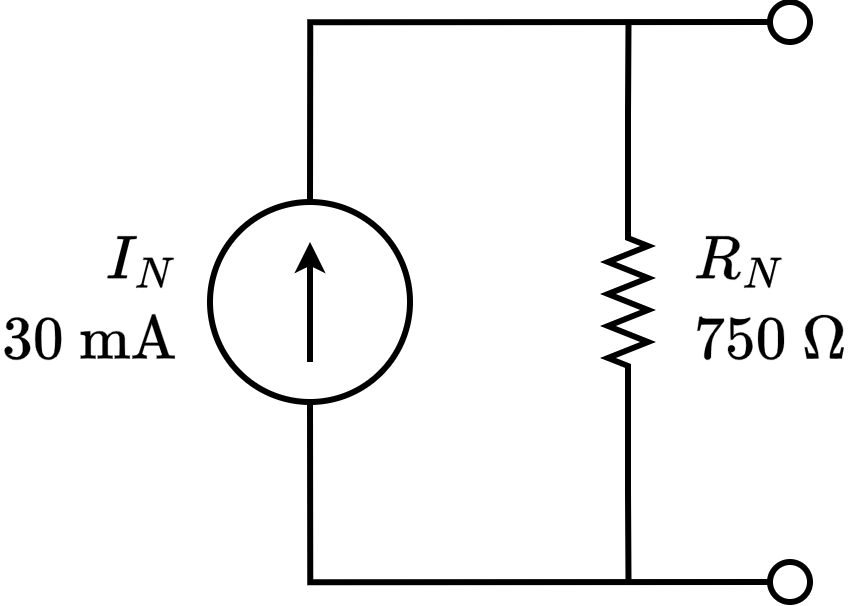
\includegraphics[width=2.2in]{questionbank/networks/ammeter_thevenin_norton/v1/norton_eq.png}
\end{center}
\end{answer}
\end{partquestion}

\begin{partquestion}{ri300}{What is the ammeter reading if $R_{i}=90~\Omega$?}
\begin{answer}
Using the Thévenin equivalent with $R_{i}=90~\Omega$ and $R_{L}=560\Omega$ gives:
\[
I_O = \frac{V_{\text{th}}}{R_{\text{th}} + R_{i} + R_{L}} = \frac{22.5}{750 + 90 + 560} \approx 16.07~\text{mA}.
\]
\end{answer}
\end{partquestion}

\begin{partquestion}{ri0}{What is the ammeter reading if $R_{i}=0~\Omega$?}
\begin{answer}
With $R_{i}=0~\Omega$ the current is:
\[
I_O = \frac{22.5}{750 + 0 + 560} \approx 17.17~\text{mA}.
\]
\end{answer}
\end{partquestion}

\begin{partquestion}{rimax}{What is the maximum value of $R_{i}$ such that the deviation in $I_O$ is less than 1\%? Find the ammeter reading with this maximum.}
\begin{answer}
Let's call the max deviation $\alpha = 0.01$. Since adding any $R_i$ reduces the total current, we wish to determine when $I_{R_i}/I_{0} \geq 1-\alpha$. Let's solve for $R_i$:
\begin{align*}
    \frac{I_{R_i}}{I_0} &\geq 1-\alpha \\
    \frac{R_{th} + R_L}{R_{th} + R_L + R_i} &\geq 1-\alpha \\
    \frac{R_{th} + R_L}{1-\alpha} &\geq R_{th} + R_L + R_i \\
    (R_{th} + R_L)(\frac{1}{1-\alpha} - 1) &\geq R_i \\
    R_i &\leq (R_{th} + R_L)\frac{\alpha}{1-\alpha} \\
    R_i &\leq (750 + 560)\frac{0.01}{0.99} \\
    R_i &\leq 13.23\unit{\ohm}
\end{align*}

Let's find $I_O$ with this new resistance:
\[
I_O = \frac{22.5}{750 + 13.23 + 560} \approx 17.00~\text{mA (nice)}
\]

\end{answer}
\end{partquestion}

\end{mainquestion}


% Problem 4 - Source Transformation Voltage Calculation (18 points)
\clearpage
\Point{sourcetransform}{findvo}{18}
\begin{mainquestion}{sourcetransform}{Source Transformations}
Use source transformations to find the voltage $V_{O}$ in the circuit below.

\begin{center}
    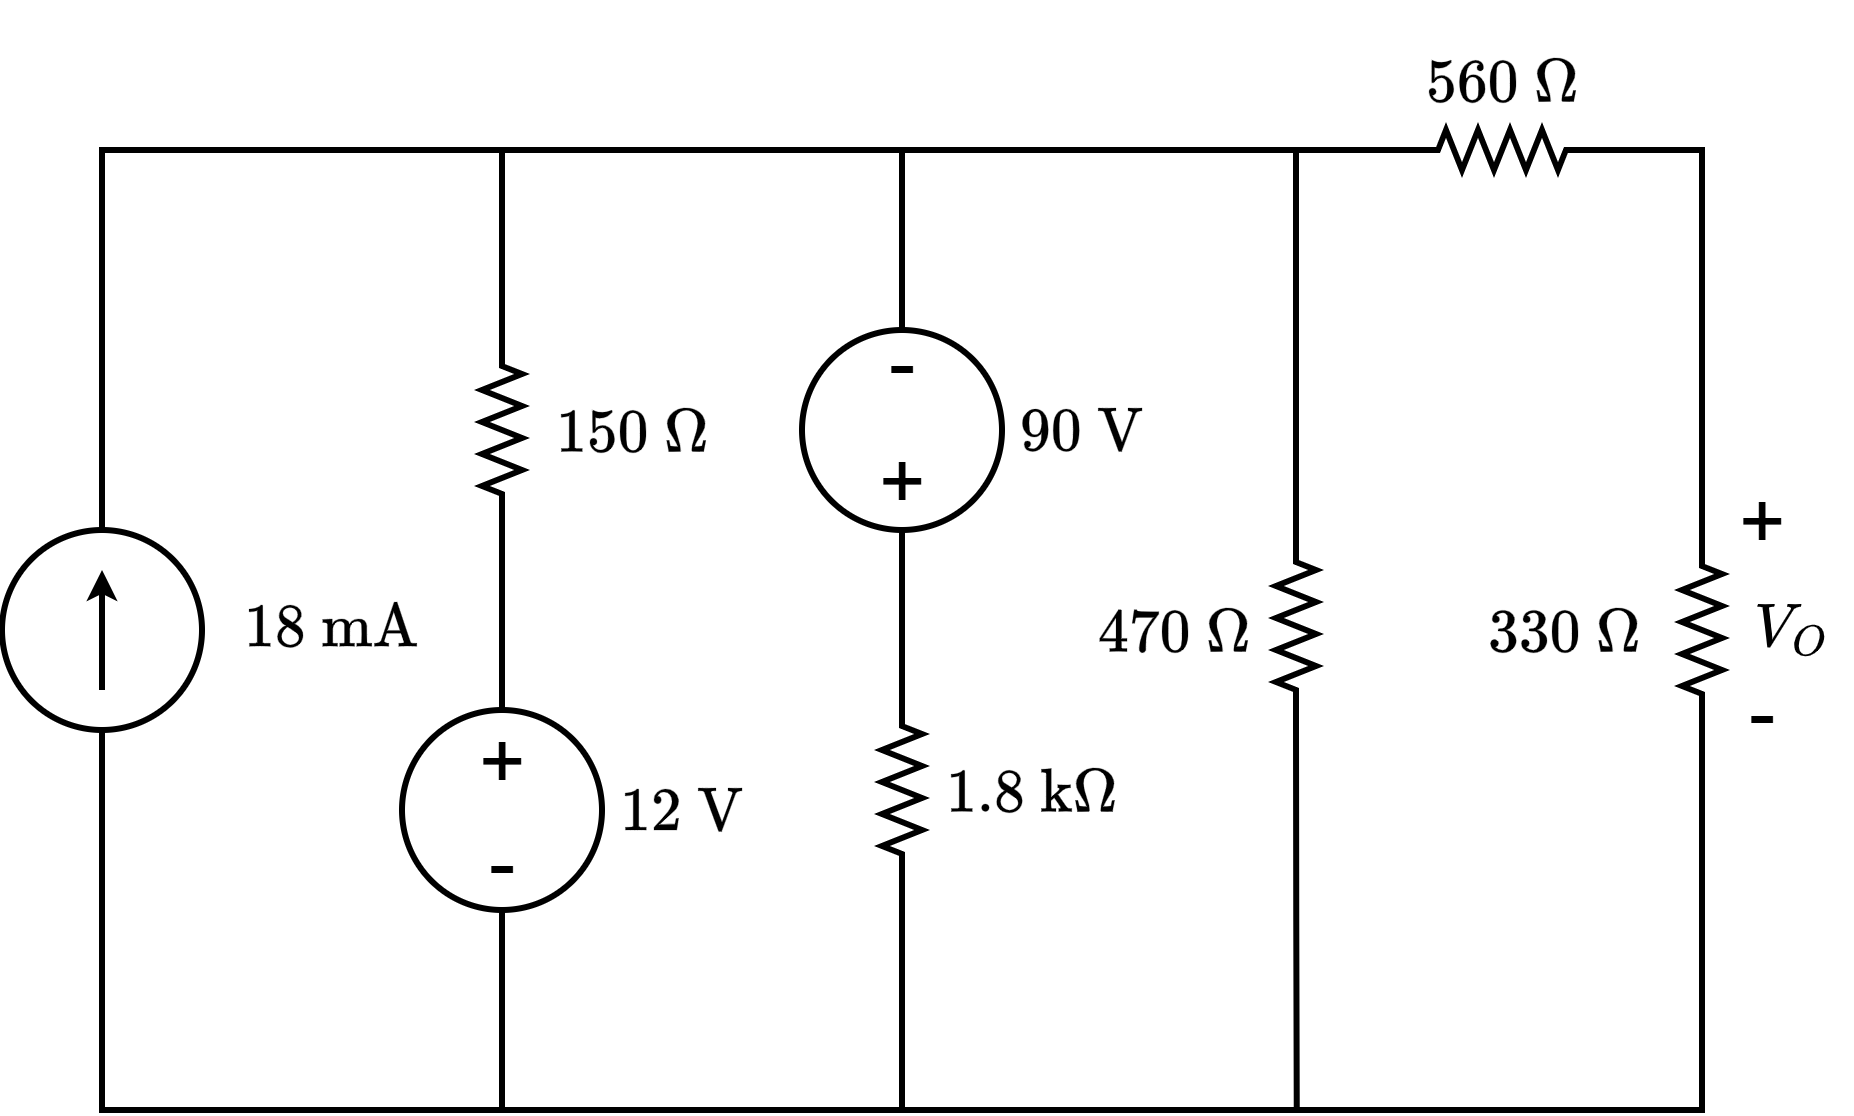
\includegraphics[width=0.8\textwidth]{questionbank/networks/source_transformations/v1/circuit.png}
\end{center}

\begin{partquestion}{findvo}{Find $V_{O}$ using source transformations.}
\begin{answer}
We first transform the 12 V source with the $150~\Omega$ series resistance into its Norton equivalent with a Norton source current of $\frac{\qty{12}{\volt}}{\qty{150}{\ohm}} = \qty{80}{\milli\ampere}$ and a Norton resistance of $150~\Omega$. Simultaneously, we can transform the 90 V source with the \qty{1.8}{\kilo\ohm} series resistance into its Norton equivalent with a Norton source current of $\frac{\qty{90}{\volt}}{\qty{1.8}{\kilo\ohm}} = \qty{50}{\milli\ampere}$ and a Norton resistance of \qty{1.8}{\kilo\ohm}. Note the polarity of the two sources are different, so the Norton current sources will be pointing in different directions! The resulting circuit looks like:

\begin{center}
    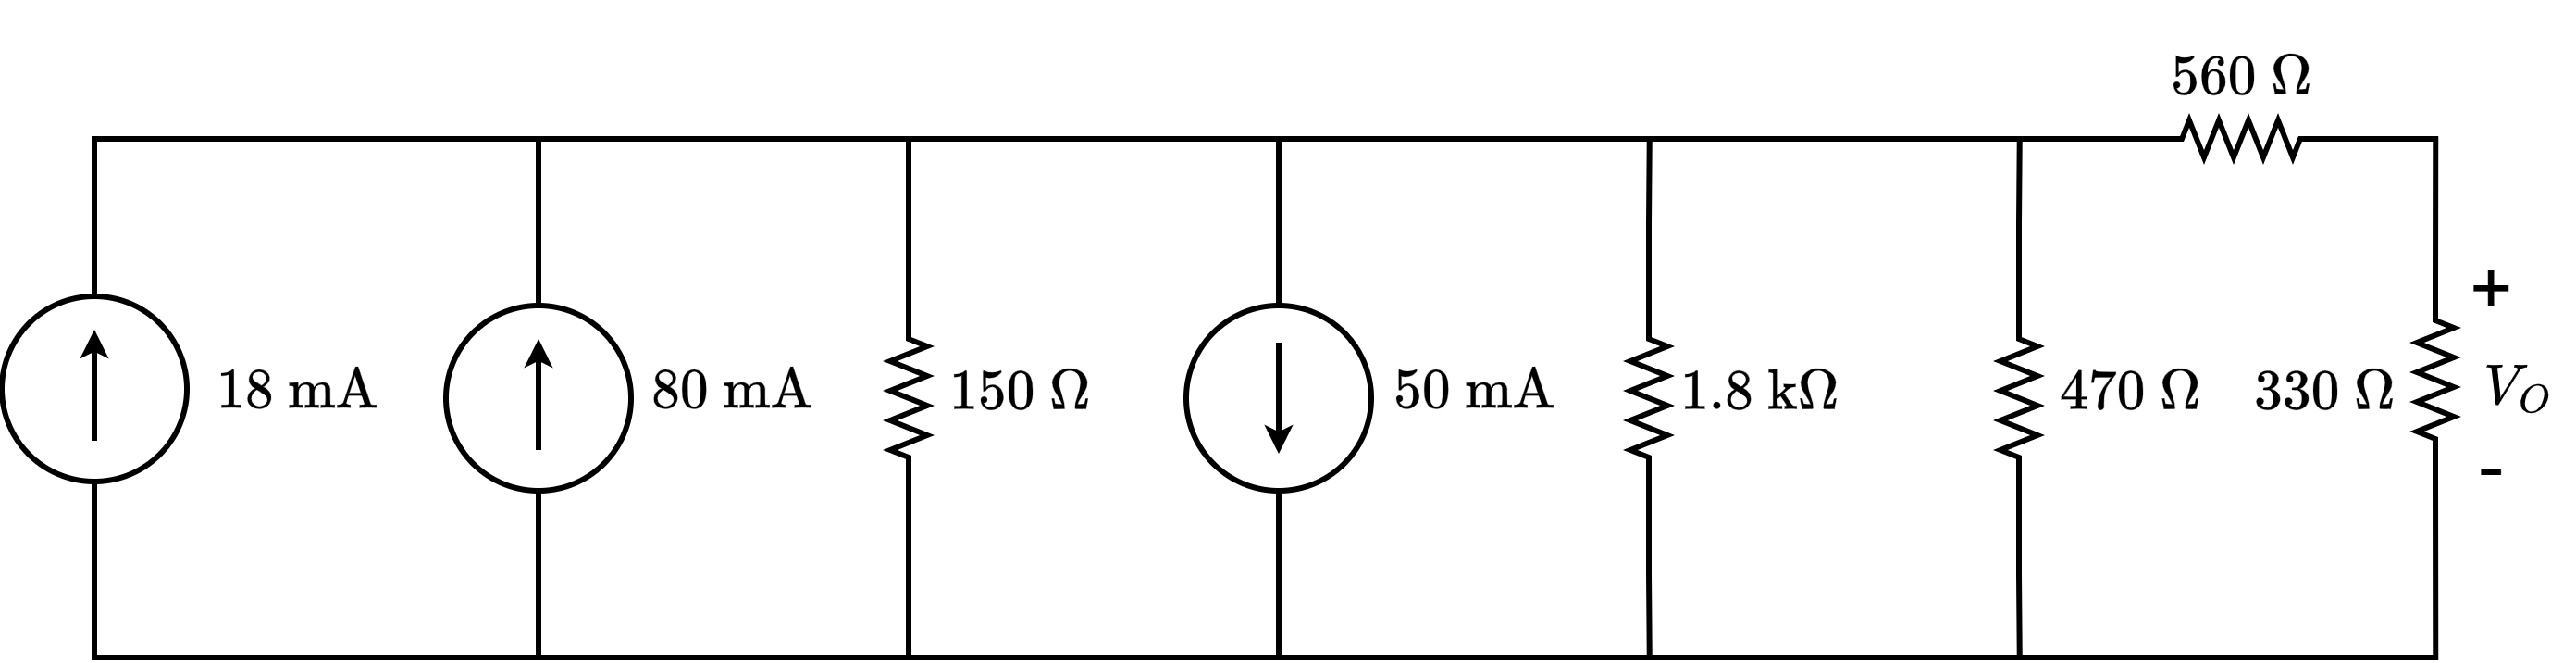
\includegraphics[width=0.8\textwidth]{questionbank/networks/source_transformations/v1/transform_1.png}
\end{center}

We can simplify the circuit considerably by combining the current sources since they are in parallel to form a \qty{48}{\milli\ampere}
source. We can also combine the three parallel resistors with a single resistor of value \qty{107}{\ohm}.
The simplified circuit looks like:

\begin{center}
    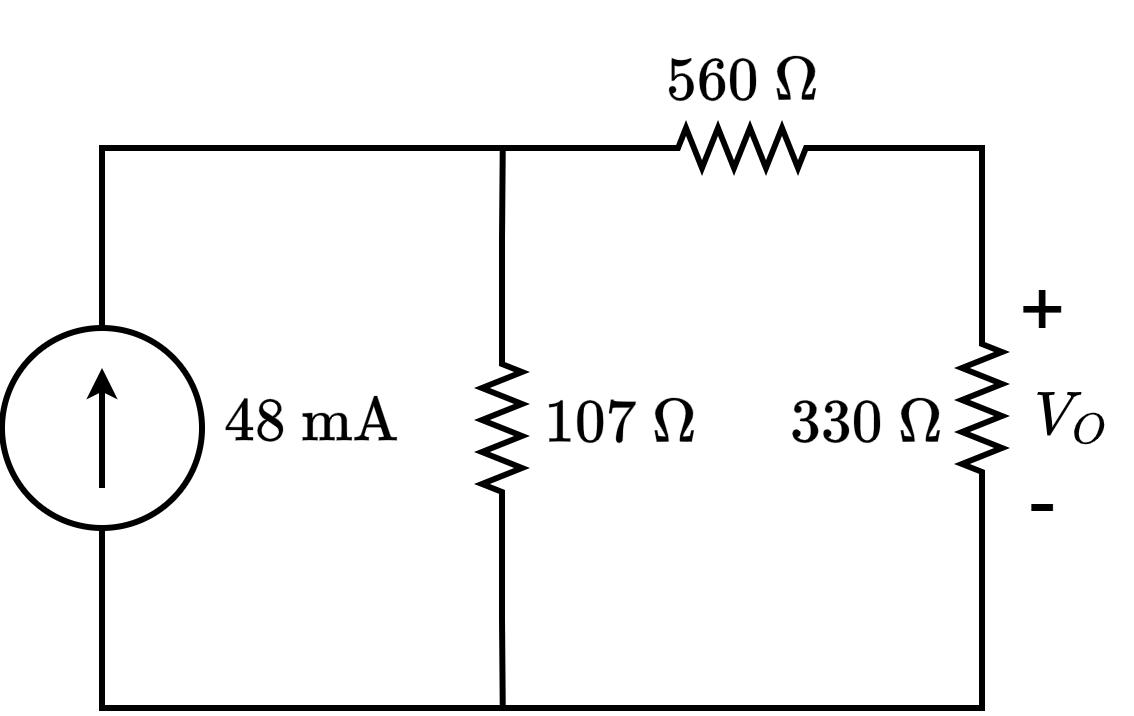
\includegraphics[width=0.5\textwidth]{questionbank/networks/source_transformations/v1/transform_2.png}
\end{center}

The next step is to apply another source transformation to a Thévenin equivalent with a Thévenin voltage source of \qty{5.13}{\volt}
with a Thévenin resistance of \qty{107}{\ohm}.
The result looks like:

\begin{center}
    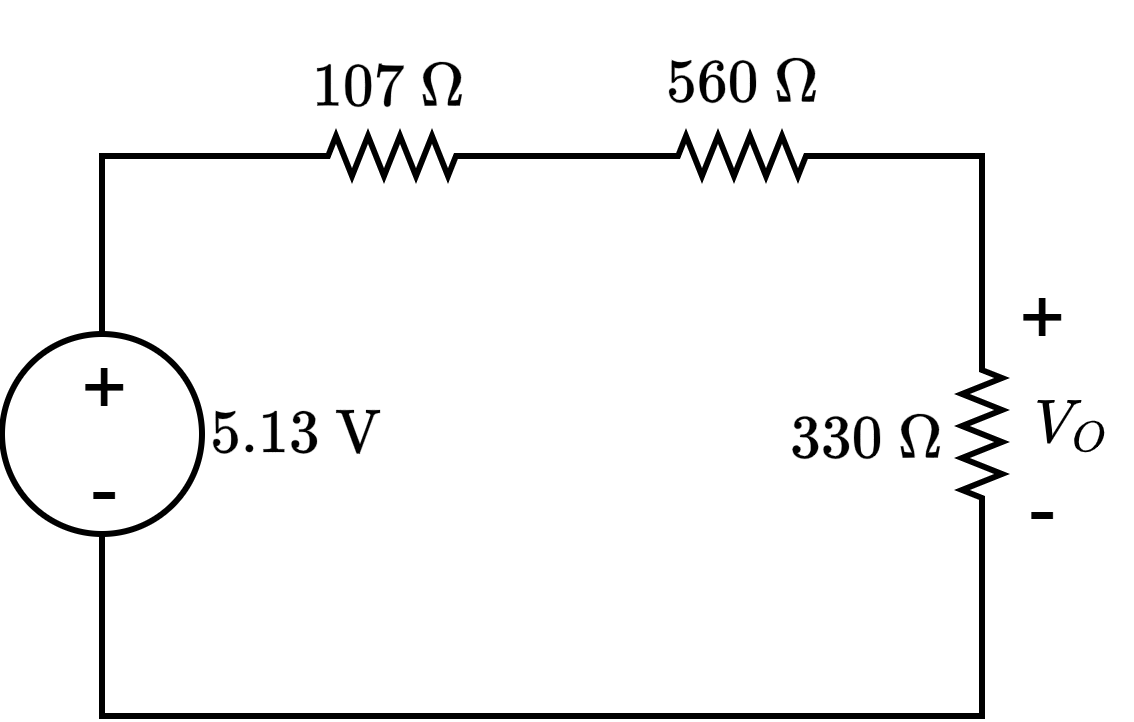
\includegraphics[width=0.5\textwidth]{questionbank/networks/source_transformations/v1/transform_3.png}
\end{center}

The result is a simple voltage divider. We can easily find the voltage across the $330~\Omega$ resistor as:
\[
V_{O}
=
5.13
\left(
\frac{330}{330+560+107}
\right)
=
\qty{1.70}{\volt}
\]
\end{answer}
\end{partquestion}

\end{mainquestion}

% Problem 5 - Battery Internal Resistance and Power Curve (10 points)
\clearpage
\Point{battery}{peakcurrent}{2}
\Point{battery}{peakpower}{4}
\Point{battery}{plotpower}{4}
\begin{mainquestion}{battery}{Power Transfer}
A typical CR2032 3 V coin-style battery (often used in watches or small electronic devices) has an internal source resistance $R_{s}$ of about $17~\si{\ohm}$ (seriously!) at room temperature. (While this value typically increases as the battery is depleted, we will consider it constant for this problem.)

\begin{center}
    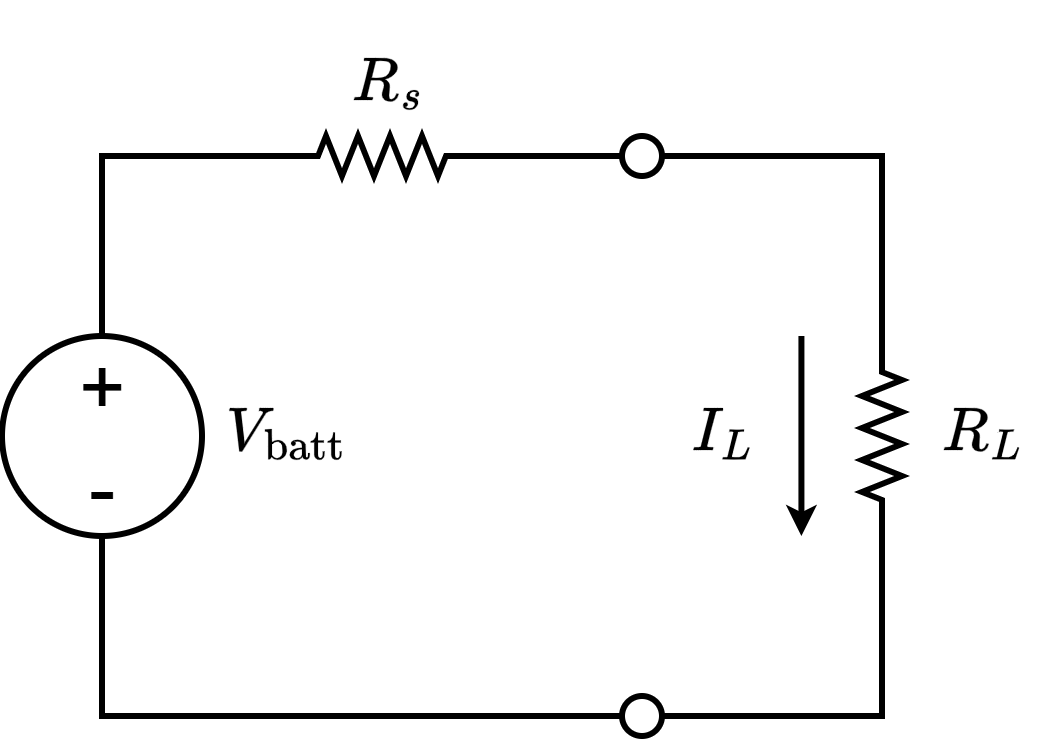
\includegraphics[width=4in]{questionbank/networks/battery_internal_resistance/v0/circuit.png
    }
\end{center}

\begin{partquestion}{peakcurrent}{Using this battery, what is the peak current that could be driven through an external load $R_{L}$? What is $R_{L}$ in this scenario?}
\begin{answer}
The current is
\[
I=\frac{V_{\text{batt}}}{R_s+R_L},
\]
and to make this as large as possible, we make the denominator as small as possible. With $R_s$ fixed, we make
\[
R_L=0,
\]
so
\[
I=\frac{V_{\text{batt}}}{R_s} = \frac{3}{17}\,\si{\ampere}
    \approx 176\,\si{\milli\ampere}.
\]
\end{answer}
\end{partquestion}

\begin{partquestion}{peakpower}{Using this battery, what is the peak power that could be delivered through an external load $R_{L}$? What is $R_{L}$ in this scenario?}
\begin{answer}
Maximum power transfer occurs when
\[
R_L=R_s=17\,\si{\ohm},
\]
and the value of the power is
\[
P= \frac{V_L^2}{R_L} = \frac{(V_{\text{batt}}\frac{R_L}{R_s + R_L})^2}{R_L} = \frac{V_{\text{batt}}^2R_L}{(R_s + R_L)^2}
= \frac{V_{\text{batt}}^2}{4R_s}
=\frac{3^2}{4(17)}
=\frac{9}{68}\,\si{\watt}
\approx132\,\si{\milli\watt}.
\]
\end{answer}
\end{partquestion}

\begin{partquestion}{plotpower}{Plot the power delivered to $R_{L}$ as a function of $R_{L}$, from $0$ to $500~\si{\ohm}$.}
\begin{answer}
In the previous part, we derived the formula for the power dissipated in the load as:
\[P_{L} = \frac{V_{\text{batt}}^{2} R_{L}}{(R_{L} + R_{s})^{2}} = \frac{9 R_{L}}{(R_{L} + 17)^{2}}.\]

This can be plotted using MATLAB or some equivalent graphing program; the figure is shown below.

\begin{center}
    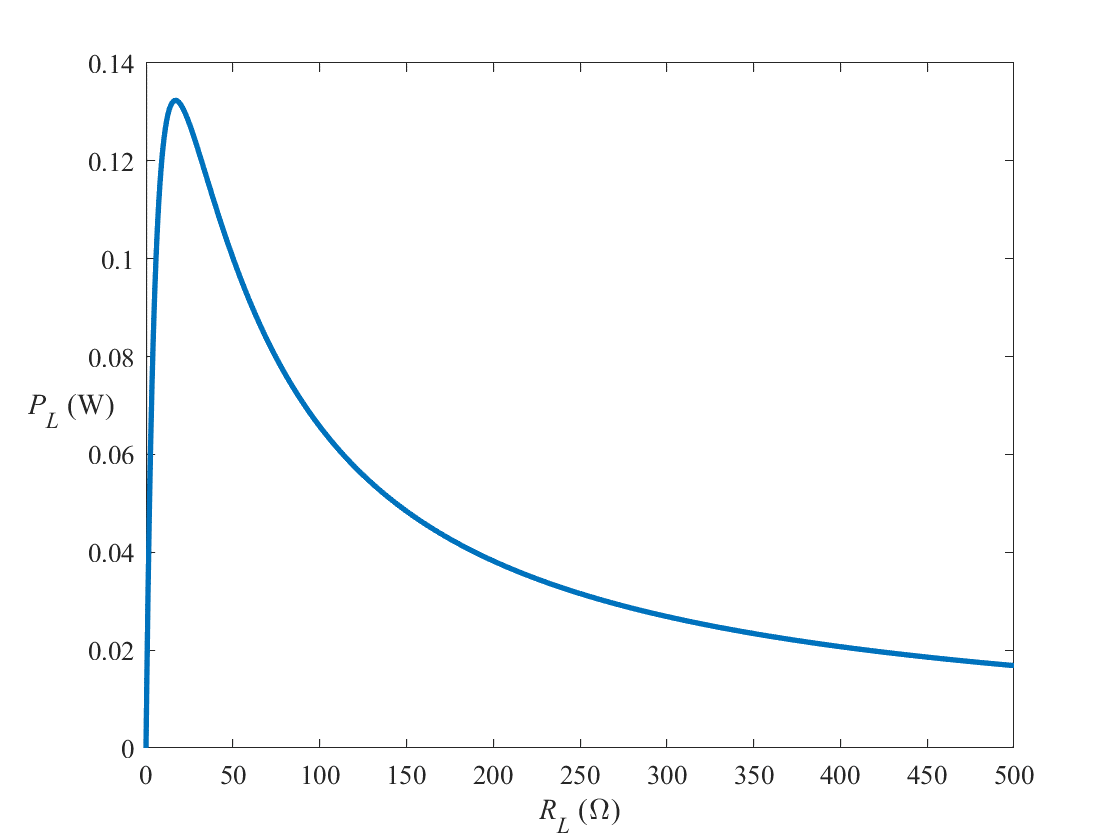
\includegraphics[width=5in]{questionbank/networks/battery_internal_resistance/v0/plot.png}
\end{center}

Note the peak occurs at $17~\si{\ohm}$, as we expect. The power delivered to the load rolls off to zero as $R_L$ goes to zero.
\end{answer}
\end{partquestion}

\end{mainquestion}